\documentclass{article}
\usepackage{listings}
\usepackage{graphicx}
\usepackage{color}
\usepackage{float}

\definecolor{dkgreen}{rgb}{0,0.6,0}
\definecolor{gray}{rgb}{0.5,0.5,0.5}
\definecolor{mauve}{rgb}{0.58,0,0.82}

\lstset{
	frame=single,
	language=C,
	belowskip=3mm,
	showstringspaces=false,
	columns=flexible,
	captionpos=b,
	basicstyle={\small\ttfamily},
	numbers=left,
	numbersep=5pt,
	%numbers=none,
	numberstyle=\tiny\color{gray},
	keywordstyle=\color{blue},
	commentstyle=\color{dkgreen},
	stringstyle=\color{mauve},
	breaklines=true,
	breakatwhitespace=true,
	tabsize=4
}

\input kvmacros
\sloppy
\begin{document}

\title{Programming Assignment 2 - N-body Simulation}
\author{\textit{Yesheng Ma}\\\textit{Ke Chang}}
\date{November 29th, 2016}
{\bf\small CS433:Parallel Programming}\hfill{\bf\small 2016 Fall}
{\let\newpage\relax\maketitle}
\maketitle


\begin{abstract}
	The n-body problem is a famous problem regarding approximating the motion of particles. The main idea is using the Newtonian gravitational force equation
	to simulate the motion. In this project, we try to parallelize the n-body simulation program and we will give a benchmark on both the serialized version
	and parallelized version.
\end{abstract}


\section{Introduction}
First let's shed a light on what n-body simulation acutally is. An N-body simulation of a dynamic system of particles, usually under the influence of physical
forces, such as gravity. The default number of particles in the system is $200$ and the user can specify the number of particles by explicitly input an argument
to	the program. Another important parameter is the number of iterations and the default value is $10000$.


\section{Implementation}
In the N-body simulation, the core function is \verb|position_step| which calculates the forces of bodies and update the positions of the bodies and 
we are going to analyze this function both on a sequential manner and parallel manner.

\subsection{Profiling of the Sequential Version}
We can use the linux tool \emph{gprof} to help us profile the execution of the n-body program. We can use following commands to get profiling information:
\begin{enumerate}
	\item \verb|gcc nbody.c -o nbody -lm -lX11 -pg|: compile the program with debug information.
	\item \verb|./nbody 1000|: execute the program so that the related debug information is generated.
	\item \verb|gprof nbody gmon.out -p|: get the profiling result of last execution.
\end{enumerate}

\begin{table}
	\centering
	\begin{tabular}{c|c}
		function name & time(s) \\ \hline
		\verb|position_step| & 4.95 \\ \hline
		\verb|collision_step| & 0.00 \\ \hline
		\verb|step_world| & 0.00 \\ \hline
		\verb|create_world| & 0.00 
	\end{tabular}
	\caption{Profile of the Sequential Version(nbody 1000, iter 200)}
\end{table}
As we can see in the above table, the execution time of function \verb|position_step| almost takes $100\%$ of the whole execution time, thus
what we are going to do is just parallelize this function.


\subsection{Sequential Version of \texttt{position\_step}}
The sequential version of function \verb|position_step| is rather simple.
What it does is update the positions of each body in this world:
\begin{enumerate}
\item Allocate memory for \verb|force_x| and \verb|force_y| and initialize them to 0.
\item Compute the force on each body. Since each body has a force on all other bodies except itself, thus this computation is a two-level loop. In the outer loop we traverse all the bodies and in the inner loop we traverse all the body except the $i$th body.
\item Update the velocity and position of each body according to related physical laws.
\end{enumerate}


\subsection{Parallel Version of \texttt{position\_step}}
The process of parallelizing the \verb|position_step| function is quite
similar to what we have done in the previous project to parallelize
Dijkstra's shortest path algorithm. The only different part is that in the
previous project, we use MPI to accomplish parallelism and this time we use
OpenMP.

The main idea is just partition all the bodies by the number of available
threads and make the computation of the force array parallelized. Also, the
computation of update position and velocity can also be parallelized
together with the computation of force. The key ideas are listed as follows:
\begin{enumerate}
	\item Use the compile-time macro \verb|#pragma omp parallel|, which will further make the following for loop run in parallel with specified thread number.
	\item Use OpenMP API \verb|omp_get_thread_num|, we can get the rank of current thread, which can be used when we partition the computation of force array.
	\item We should take care of the index of force array since we do not want different threads to handle the same memory space. Here we introduce a local variable \verb|loc_i| and we can get the global index by adding this local index to the base index of this thread.
	\item Another important note is that we should try to make variables 
		local to achieve high performance. For example, when you write
		a for loop and you define the index \verb|i| outside OpenMP macro,
		then the performance will be quite bad. If you declare this variable
		inside OpenMP macro, you will gain much better performance.
\end{enumerate}

The code for \verb|position_step| is shown as follows:
\begin{lstlisting}[language=C]
  /* Compute the net force on each body */
#	pragma omp parallel num_threads(thread_count)
{
	int i, j, loc_i;
	double d, d_cubed, diff_x, diff_y;
	int my_rank = omp_get_thread_num();
	int loc_num_bodies = world->num_bodies / thread_count;
	int loc_base_idx = my_rank * loc_num_bodies;

	for (loc_i = 0; loc_i < loc_num_bodies; ++loc_i) {
		for (j = 0; j < world->num_bodies; ++j) {
			i = loc_base_idx + loc_i;
			if (i == j)
				continue;
			// Compute the x and y distances and total distance d between
			// bodies i and j
			diff_x = world->bodies[j].x - world->bodies[i].x;
			diff_y = world->bodies[j].y - world->bodies[i].y;
			d = sqrt((diff_x * diff_x) + (diff_y * diff_y));

			if (d < 25) {
				d = 25;
			}
			d_cubed = d * d * d;
			// Add force due to j to total force on i
			force_x[i] += GRAV * (world->bodies[i].m * world->bodies[j].m
					/ d_cubed) * diff_x;
			force_y[i] += GRAV * (world->bodies[i].m * world->bodies[j].m
					/ d_cubed) * diff_y;
		}
	}
	
	// Update the velocity and position of each body
	for (loc_i = 0; loc_i < loc_num_bodies; loc_i++) {
		i = loc_base_idx + loc_i;

		// Update velocities
		world->bodies[i].vx += force_x[i] * time_res / world->bodies[i].m;
		world->bodies[i].vy += force_y[i] * time_res / world->bodies[i].m;		
		
		// Update positions
		world->bodies[i].x += world->bodies[i].vx * time_res;
		world->bodies[i].y += world->bodies[i].vy * time_res;
	}	
}
\end{lstlisting}

\subsection{A Few Words about Optimizing the Performance}
I think the most important optimization we have done to get better performance is to make some variables local to OpenMP.
We refer to some documentations and find that if you use a non-local variable in OpenMP, OpenMP will create a data structure
with lock related to that non-local data structure. Since this is not a memory intensive program, we tend to make each thread use
its own memory and in this way OpenMP will naturally use a lock-free data structure to hold those variables.

Before doing the optimization, the OpenMP program runs roughly at the speed of original serial version and after the optimization
the program begins to benefit from parallelism.



\subsection{The Barnes-Hut Algorithm to Speed Up}
The Barnes-Hut simulation is an approximation algorithm for performing an
n-body simulation. It has a much lower time complexity of $O(n\log n)$,
compared with the original brute-force computation which is of time
complexity $O(n^2)$. And we can see that this change is actually a significant
difference.

The major idea of the Barnes-Hut algorithm is to model the distrubution of
all the particles by a data structure called Barnes-Hut Oct-tree, quad tree for short. This tree
is quite similar to a binary tree but in a quad tree, each node can have four child nodes,
which represents northwest, northeast, southwest and southeast respectively.

In order to calculate force on a particle, we need to construct the tree first. This process
is not very hard, since real particles can only be put on the leaf nodes of a quad tree.
We insert all the particles into this quad tree, on inserting each node, we first check if
this node is a leaf node. If so, we directly write to this node; otherwise, we update the
information about the mass center of this subtree and insert this particles to one of the four directions.
This is a recursive procedure and the in the final state each particle resides in a leaf.

Next, we calculate the force on each particle. To calculate the force on each particle, we walk
through the whole quad tree:
\begin{enumerate}
\item If the current mass center satisfies a threshold, we no longer calculates the force of
	the subtree but instead use the mass center to estimate the while subtree
\item Otherwise, we still need to traverse through the whole subtree.
\end{enumerate}
In this way, we finish one iteration and the whole process is just repeat this iteration for \verb|niter| times.



\section{Benchmark of N-body Programs}
In this section, we will show the result we run both on PC and cluster.
\subsection{Brute-force \& Its Parallelized Version}
\begin{figure}[H]
\centering
	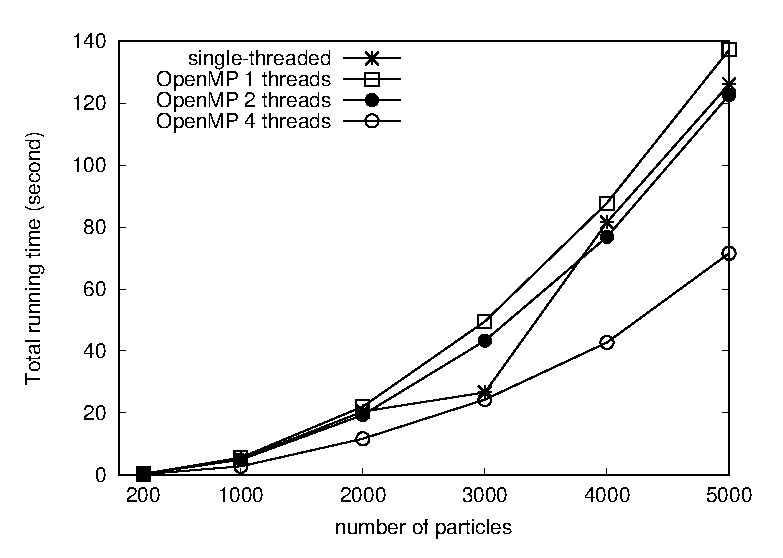
\includegraphics[width=8cm]{fig/scale_out.eps}
	\caption{Scale out of different versions of n-body on laptop}
\end{figure}

\subsubsection{Scale-up}
As we have analyzed, the time complexity of brute-force n-body simulation
should follow the order $O(n^2)$. From the above figure, we can see that
all the lines seem to satisfy a $n^2$ increasing and is consistent with
our previous knowledge.

\subsubsection{Scale-out}
What we want to emphasize on is the scale-out part since we are using
OpenMP to parallelize the algorithm. We have the following discoveries:
\begin{enumerate}
\item OpenMP produces quite efficient code when the thread number is intentionally set to 1, compared with the original code.
\item The sequential version is surprisingly efficient when dealing with $3000$ number of points. The reason for this efficiency may result from full usage of cache memory.
\item The execution time of the 4 thread version is roughly half of the single-threaded version, which is a huge improvement.
\end{enumerate}





\subsection{Running N-body on Pi}
We also run the n-body simulation on Pi supercomputer and we achieved quite good scale-out performance.
\begin{figure}[H]
	\centering
	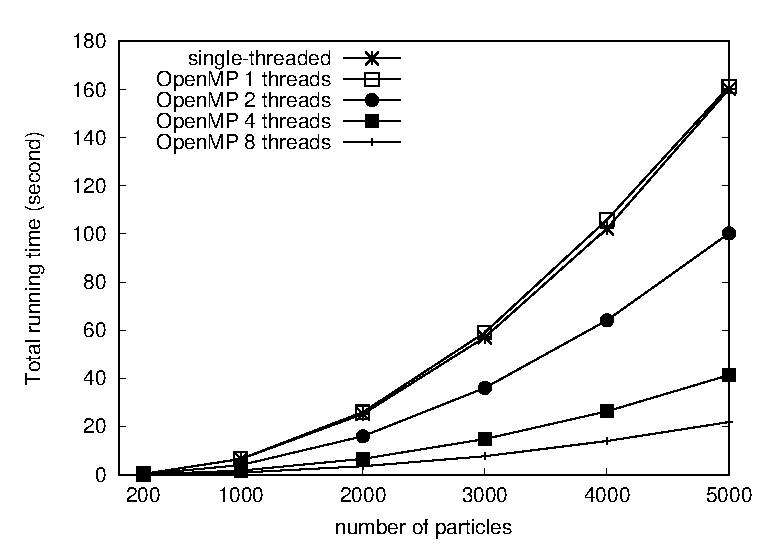
\includegraphics[width=8cm]{fig/pi_scale_out.eps}
	\caption{Scale out of different versions of n-body on Pi}
\end{figure}
What is important is that we almost get linear scale-out performance. I also have some experience programming in Spark platform,
but as far as I know, Spark cannot have such fine scale out performance. That maybe the reason why there are still so many people
using MPI and OpenMP.

The speedup rate is also listed as follows:

\begin{table}[H]
\centering
	\begin{tabular}{c|c|c|c|c}
	nbody	& 1 thread & 2 thread & 4 thread & 8 thread \\ \hline
	200		& 0.81 & 1.63 & 3.25 & 6.50 \\ \hline
	1000	& 0.99 & 1.63 & 3.83 & 7.36 \\ \hline
	2000    & 0.97 & 1.57 & 3.87 & 7.17 \\ \hline
	3000    & 0.96 & 1.58 & 3.85 & 7.25 \\ \hline
	4000	& 0.97 & 1.60 & 3.87 & 7.31 \\ \hline
	5000	& 0.99 & 1.60 & 3.87 & 7.32
	\end{tabular}
	\caption{N-body programs with different \# of threads(niter 200)}
\end{table}

\subsection{Result of the Barnes-Hut Algorithm}
We also did some expriments on the Barnes-Hut Algorithm and here we just list them as a table:
\begin{table}[H]
\centering
	\begin{tabular}{c|c|c|c}
	nbody	& 1 thread & 2 thread & 4 thread \\ \hline
	200		& 0.57 & 0.43 & 0.40  \\ \hline
	1000	& 10.59 & 7.03 & 4.93  \\ \hline
	2000    & 33.14 & 21.08 & 14.22 
	\end{tabular}
	\caption{N-body programs with different \# of threads(niter 200)}
\end{table}





\section{Conclustion}
To conclude, in this project we learn some basic primitives of OpenMP programming and carry out some expriments on Pi supercomputer to get a better understanding of it. As a result, the programs scale out nicely and show the power of OpenMP.

\section*{Acknowledgement}
Thanks Prof. Deng for guidance on OpenMP programming and TAs for configuring cluster and kindly answering questions.
\end{document}
